\documentclass{weekly}
\begin{document}
\maketitlew{Аналитическая механика}{2}{8}{29}

\paragraph{11.8.6.} Найти компоненты тензора инерции в~главных
центральных осях для~однородного полого цилиндра массы~$M$
с~внешним радиусом~$R_2$ и~внутренним радиусом~$R_1$.
\emph{Высота цилиндра также известна и~равна~$H$.}

$\blacktriangleright$ Направим ось~$z$ вдоль оси цилиндра~$\mathcal{V}$
и~найдём компоненты тензора инерции в~заданном таким образом
ортонормированном базисе. Если результат получится диагональным,
задача будет полностью решена.

Итак,
\begin{align}
    \hat J &= \rho \bigintsss_{\mathcal{V}}
            \begin{pmatrix}
                y^2 + z^2 & -xy & -xz \\
                -xy & x^2 + z^2 & -yz \\
                -xz & -yz & x^2 + y^2
            \end{pmatrix} dV
        =\\[2ex]&= \rho
            \bigintsss\limits_{R_1~~~}^{~~~R_2}    \!\!\!\!\!
            \bigintsss\limits_{0~~~}^{~~~2\pi}     \!\!\!\!\!\!\!
            \bigintsss\limits_{-H/2~~~}^{~~~H/2}
            \begin{pmatrix}
                r^2 \sin^2\varphi + z^2
                    & -r^2 \sin\varphi \cos\varphi
                    & -r \cos\varphi z \\
                -r^2 \sin\varphi \cos\varphi
                    & r^2 \cos^2\varphi + z^2
                    & -r \sin\varphi z \\
                -r \cos\varphi z
                    & -r \sin\varphi z
                    & r^2
            \end{pmatrix} r \,dr \,d\varphi \,dz
        =\\[2ex]&= \frac{M}{\pi H \left(R_2^2 - R_1^2\right)} \cdot 2\pi
            \bigintsss\limits_{R_1~~~}^{~~~R_2}    \!\!\!\!\!
            \bigintsss\limits_{-H/2~}^{~~~H/2}
            \begin{pmatrix}
                \frac12 r^2 + z^2 & 0 & 0 \\
                0 & \frac12 r^2 + z^2 & 0 \\
                0 & 0 & r^2
            \end{pmatrix} r \,dr \,dz
        =\\[2ex]&= \frac{2M}{H \left(R_2^2 - R_1^2\right)}
            \int\limits_{R_1}^{R_2} r \,dr
            \int\limits_{-H/2}^{H/2}
            \diag{\frac{r^2}{2}+z^2}{\frac{r^2}{2}+z^2}{r^2} dz
        =\\[2ex]&= \frac{2M}{R_2^2 - R_1^2}
            \int\limits_{R_1}^{R_2}
            \diag{\frac{r^3}{2}+\frac{H^2}{12}r}
                 {\frac{r^3}{2}+\frac{H^2}{12}r}{r^3} \,dr
        =\\[3ex]&= M \diag{\frac{R_1^2 + R_2^2}{4} + \frac{H^2}{12}}
                 {\frac{R_1^2 + R_2^2}{4} + \frac{H^2}{12}}
                 {\frac{R_1^2 + R_2^2}{2}}.
\end{align}

\bigskip
\textbf{Ответ:}\qquad
$I_{xx} = I_{yy} = M\dfrac{R_1^2+R_2^2}{4} + M\dfrac{H^2}{12}$, \quad
$I_{zz} = M\dfrac{R_1^2+R_2^2}{2}$.
\hfill $\blacktriangleleft$


\clearpage
\begin{wrapfigure}[7]{r}{.165\textwidth}
    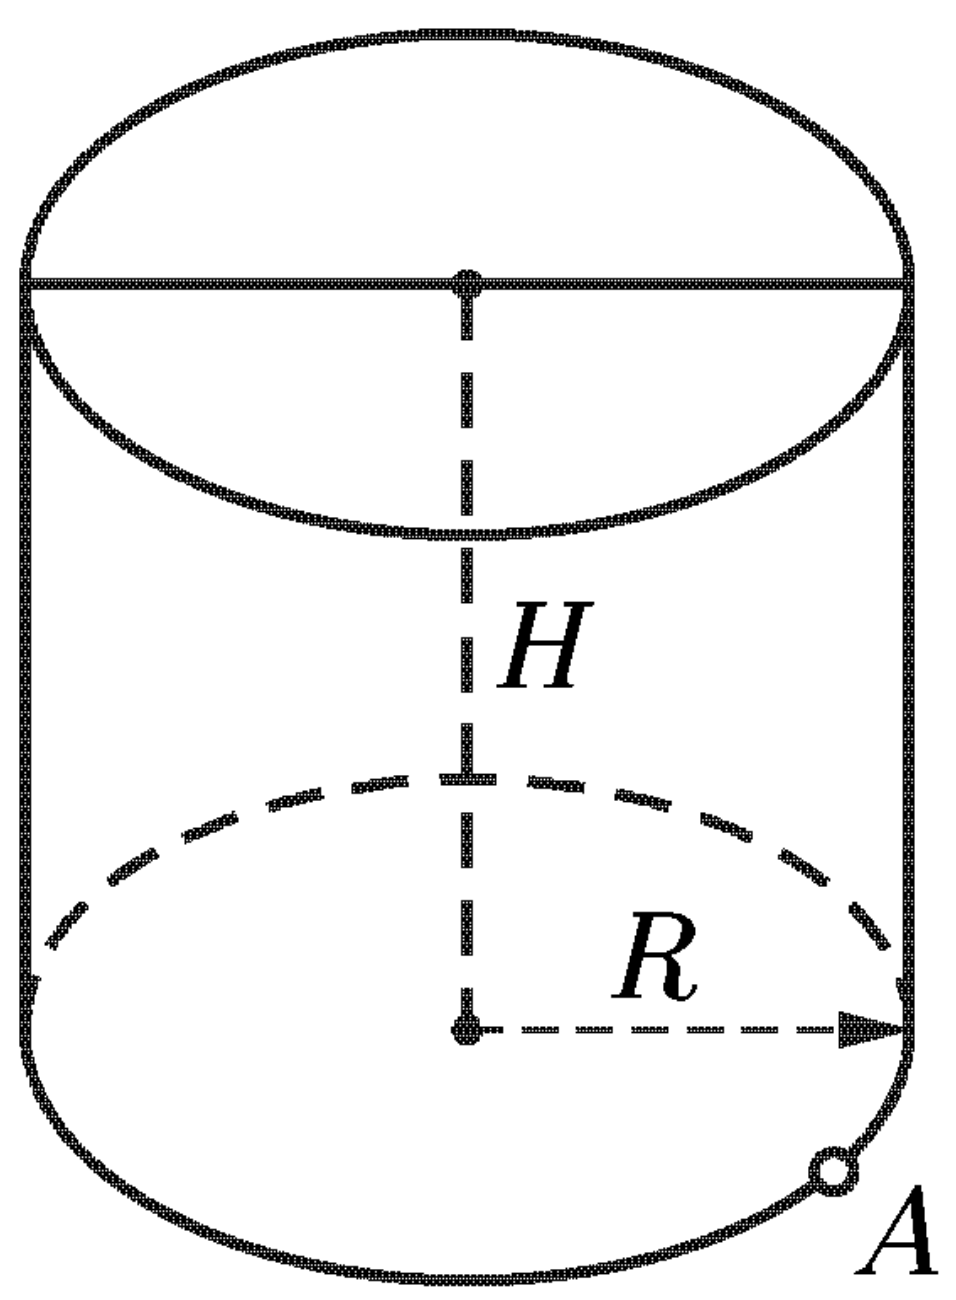
\includegraphics[width=\linewidth]{11-11}
\end{wrapfigure}
\paragraph{11.11.} Найти главные оси инерции в~точке~$A$ однородного
прямого кругового цилиндра массы~$m$. Высота цилиндра равна~$H$,
радиус основания равен~$R$. Для~случая $H = \sqrt{3} R$ выписать
тензор инерции цилиндра в~главных осях для~точки~$A$.

$\blacktriangleright$ Применим теорему Гюйгенса--Штейнера,
полагая тензор инерции цилиндра в~центральных главных осях известным
\emph{(хотя~бы положив~$R_1 = 0$ в~11.8.6),} направив
ось~$Ox$ вдоль полярной плоскости точки~$A$ и~выполнив параллельный
перенос начала отсчёта в~$A$:
\begin{gather}
    \overline{AO} = \left(-R; \; 0; \; \dfrac{H}{2}\right);
\\
    \hat J_A = M
            \begin{pmatrix}
                \frac{1}{4} R^2 + \frac{1}{3} H^2 & 0 & \frac{1}{2} RH \\
                0 & \frac{5}{4} R^2 + \frac{1}{3} H^2 & 0 \\
                \frac{1}{2} RH & 0 & \frac{3}{2} R^2
            \end{pmatrix}.
\end{gather}
Поскольку дальше будет плохо, подставлю сразу~$H = \sqrt{3}R$:
\begin{equation}
    \hat J_A = \frac{MR^2}{4}
            \begin{pmatrix}
                5 & 0 & 2\sqrt{3} \\
                0 & 9 & 0 \\
                2\sqrt{3} & 0 & 6
            \end{pmatrix}.
\end{equation}
Эту матрицу неплохо было~бы диагонализировать. Для~этого вспомним
курс линейной алгебры и~начнём искать её собственные числа
и~собственные векторы. \emph{Этот процесс я, конечно, опущу.}
\begin{gather}
    \hat J_A^\pi = \frac{MR^2}{4} \diag{2}{9}{9},
\end{gather}
главные оси направлены вдоль собственных векторов, из~которых
составим матрицу:
\begin{equation}
    \mathcal{M} \equiv \left(\vec x', \vec y', \vec z'\right)
        = \begin{pmatrix}
            \frac{-2\sqrt{3}}{3} & 0 & \frac{\sqrt{3}}{2} \\
            0 & 1 & 0 \\
            1 & 0 & 1
        \end{pmatrix}.
    \label{11.11:M}
\end{equation}
Нетрудно убедиться, что ось~$y' \parallel y$, то~есть одна из~найденных
главных осей касается окружности, лежащей в~основании цилиндра.

Угол между осью~$x'$ и~$z$ есть
\begin{equation}
    \arccos \frac{1}{\abs{\vec x'}} = \arccos \frac{\sqrt{21}}{7}
        \simeq 49^\circ,
\end{equation}
что~согласуется с~авторским ответом к~задаче при~$H = \sqrt{3}R$.

\textbf{Ответ:}
главные оси направлены вдоль собственных векторов, из~которых
составлена матрица~$\mathcal{M}$~--- см.~\eqref{11.11:M};
в~этих осях тензор инерции относительно точки~$A$ имеет вид
$\hat J_A^\pi = MR^2/4 \diag{2}{9}{9}$.
\hfill $\blacktriangleleft$


\clearpage
\begin{wrapfigure}[6]{r}{.2\textwidth}
    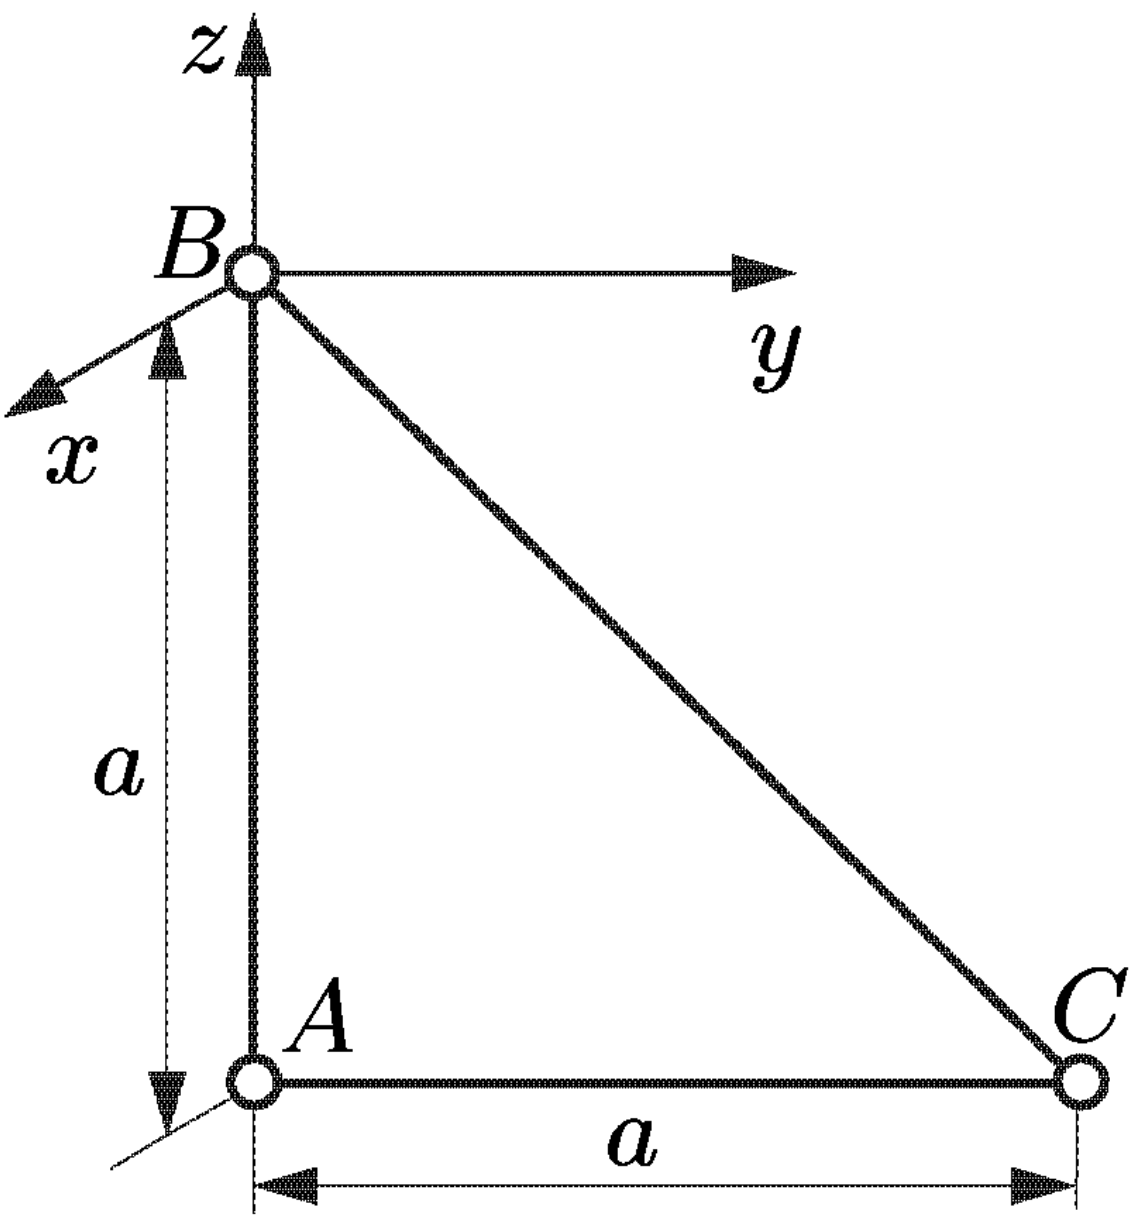
\includegraphics[width=\linewidth]{11-92}
\end{wrapfigure}
\paragraph{11.92.} Материальные точки~$A$, $B$ и~$C$ массы~$m$ каждая
находятся в~вершинах невесомого равнобедренного прямоугольного
треугольника с~длиной катета, равной~$a$. Найти тензор инерции системы
для~точки~$B$ в~указанных на~рисунке осях. Найти главные оси
для~точки~$B$. Показать, что~эллипсоид инерции для~точки~$A$
является эллипсоидом вращения.

$\blacktriangleright$ По~определению:
\begin{align}
    \hat J_A &= ma^2 \begin{pmatrix}
        2 & 0 & 0 \\
        0 & 1 & 0 \\
        0 & 0 & 1
    \end{pmatrix};
&
    \hat J_B &= ma^2 \begin{pmatrix}
        3 & 0 & 0 \\
        0 & 2 & 1 \\
        0 & 1 & 1
    \end{pmatrix}.
\end{align}
Аналогично~11.11, выпишем матрицу собственных векторов~$\hat J_B$.
Вдоль них направлены искомые оси.
\begin{equation}
    \mathcal{M} = \begin{pmatrix}
        1 & 0 & 0 \\
        0 & \frac{1 + \sqrt{5}}{2} & \frac{1 - \sqrt{5}}{2} \\
        0 & 1 & 1
    \end{pmatrix}.
\end{equation}
\emph{Процедура сама по~себе очень простая, хотя и~требующая
некоторой аккуратности.}
\hfill $\blacktriangleleft$


\paragraph{T2.} Полярным моментом инерции относительно некоторой
точки~$O$ называется величина, равная сумме произведений масс
точек системы на~квадраты их расстояний до~точки~$O$.
Показать, что~центр масс системы можно определить как~такую
точку пространства, для~которой полярный момент инерции имеет
наименьшее значение.

$\blacktriangleright$ Рассмотрим систему из~$N$ материальных точек
массами~$m_\nu$, положениям которых соответствуют
радиусы"=векторы~$\vec r_\nu$, где~$\nu = 1, \ldots, N$.
Запишем выражение для~полярного момента инерции относительно
некоторой точки~$O \to \vec r_0$ и~зададимся целью исследовать его
на~экстремум:
\begin{equation}
    \pdd{}{\vec r_0} \sum\limits_{\nu = 1}^{N} m_\nu
            \left( \vec r_\nu - \vec r_0 \right)^2
        = \pdd{}{\vec r_0} \sum\limits_{\nu = 1}^{N} m_\nu
            \left( r_\nu^2 + r_0^2 -
            2\left(\vec r_\nu,\vec r_0\right) \right)
        = 2\sum\limits_{\nu = 1}^{N} m_\nu
            \left( \vec r_0 - \vec r_\nu \right) = 0.
\end{equation}
Из~последнего равенства непосредственно вытекает, что~$\vec r_0$
есть радиус"=вектор центра масс системы (согласно известному
определению). \qed

\end{document}
